\graphicspath{{./Ch2-AnalyticalFw/images/}}

\chapter{Analyzing Off-chip Memory Accesses} \label{chap:analyticalFw}
The off-chip memory bandwidth often limits the performance of NN accelerators, and their high energy consumption also results from the large volume of off-chip memory accesses. NN accelerators use on-chip memories and reuse the data from it to minimize the number of off-chip memory accesses. Assuming that the data movement energy primarily depends on the number of bytes accessed from the memory, Figure~\ref{fig:memsAccess} illustrates the impact of data reuse from the on-chip memory on data movement energy. Figure~\ref{fig:memsAccessSingle} and Figure~\ref{fig:memsAccessDouble} show the number of memory accesses and energy estimates when data is directly accessed from the off-chip memory and when reusing the data from on-chip memory, respectively. Let $N$ is the number of bytes accessed by the processing element (PE), and $e_{1}$ and $e_{2}$ are the energy per byte access from the off-chip and on-chip memories, respectively. If $E_1$ is the data movement energy when PE accesses $N$ bytes of data directly from off-chip memory (Figure~\ref{fig:memsAccessSingle}), $E_1$ can be expressed as following
\begin{equation}\label{eq:E_1} 
	E_{1}= N\cdot e_1
\end{equation}
Let $E_2$ is the data movement energy when two levels of memory are used (Figure~\ref{fig:memsAccessDouble}) and $n$ is the data reuse from the on-chip memory per byte of off-chip memory access. In this two-level of memory hierarchy Figure~\ref{fig:memsAccessDouble}, although the total number of bytes accessed by PE is still the same ($N$), the number of off-chip memory accesses is reduced to $\frac{N}{n}$. The data movement energy ($E_2$ ) in this case can be expressed as follows,
\begin{align}\label{eq:E_2}
	\begin{split}
	E_{2}&= \frac{N}{n}\cdot e_1 + \frac{N}{n}\cdot n\cdot e_2 \\
	&= N\cdot e_1\cdot (\frac{1}{n}+ \frac{e_2}{e_1})
	\end{split}
\end{align}
The energy efficiency compared to (Figure~\ref{fig:memsAccessSingle}) can be expressed as, 
%\begin{equation}\label{eq:e_efficiency} 
%	E_{efficiency}=1-\frac{E_2}{E_1}=1-(\frac{1}{n}+\frac{e_{2}}{e_{1}})
%\end{equation}
\begin{align}\label{eq:e_efficiency}
	\begin{split}
	E_{efficiency}&=1-\frac{E_2}{E_1}\\
	&=1-(\frac{1}{n}+\frac{e_{2}}{e_{1}})
	\end{split}
\end{align}
For a given architecture, $e_{1}$ and $e_{2}$ are fixed and $e_1$ is significantly high compared to $e_2$. Equation~\ref{eq:e_efficiency} shows energy efficiency improves significantly with data reuse from the lower memory level ($n$). DNN accelerators use multiple levels of on-chip memories and apply techniques to maximize the data reuse from the lower memories to improve energy efficiency. 
\begin{figure}[!htb]
	\centering
	\captionsetup{font=sf}
	\subfloat[]{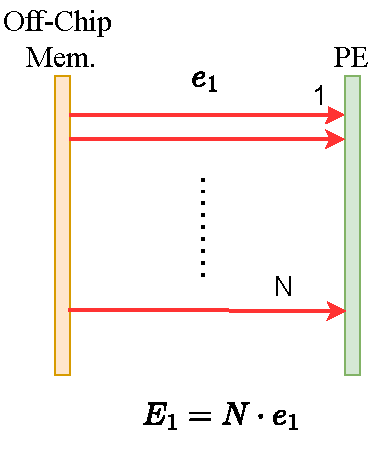
\includegraphics[width=0.25\textwidth]{memAccessSingleLevel}
		\label{fig:memsAccessSingle}}
	\hfil	
	\subfloat[]{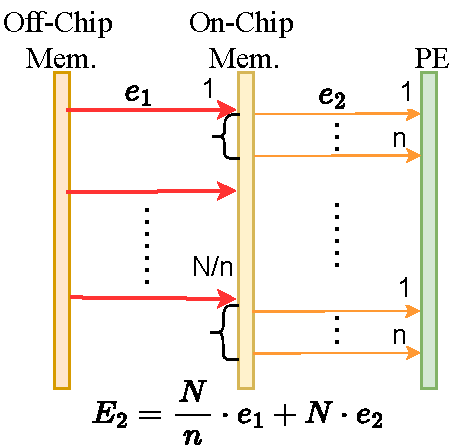
\includegraphics[width=0.3\textwidth]{memAccess2Level.pdf}
		\label{fig:memsAccessDouble}}
	\hfil	
	\caption{Memory accesses and energy estimates for accessing data (a) always from the off-chip memory. (b) from two-level of memory hierarchy while reusing the data from on-chip memory.}
	\label{fig:memsAccess}
\end{figure}

The NN accelerator reads the input data (or input activations), filter weights, and partial sums from the off-chip memory and stores them temporarily in the on-chip memory. The PE array reads the data from the on-chip memory to perform the computations and then stores them back to the on-chip memory. The partial sums or the outputs of the computations are then finally stored in the off-chip memory. The data flow is shown in Figure~\ref{fig:nnDataFlow}. Due to the significant difference between the energy consumption of accessing the data from the off-chip memory and the on-chip memory, NN accelerators aim to minimize the off-chip memory accesses by exploiting the memory hierarchy and data reuse from them.
\begin{figure}[!htb]
	\centering
	\captionsetup{font=sf}	
	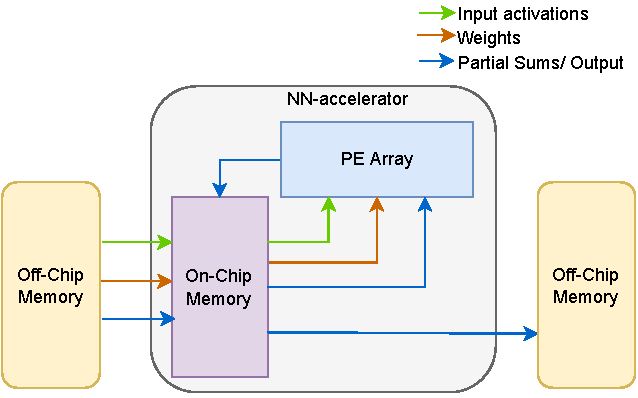
\includegraphics[width=0.5\textwidth]{nnDataFlow}
	\caption{Read/Write of inputs, weights and partial/final outputs from different level of memories.}
	\label{fig:nnDataFlow}
\end{figure}

The layer data is stored as multi-dimensional arrays in the off-chip memory, which is generally too large to fit in the local on-chip memory. In order to perform the computations, the large layer data is partitioned into small tiles. These tiles are repeatedly fetched from the off-chip memory to compute the final output sum. To observe the impact of tile dimensions on off-chip memory accesses for a given data reuse scheme, we measured the off-chip memory accesses for a popular CNN, VGG16, for different tile dimensions using the algorithm described in section~\ref{sec:Access3DData}. Figure~\ref{fig:impactOfTileDims} shows the impact of tile dimensions on off-chip memory accesses for VGG16, for a given tile scheduling scheme. Figure~\ref{fig:varyingTileDims} shows that using different tile dimensions results in different volumes of off-chip memory accesses. A good tile dimension can reduce off-chip memory accesses up to 90\% compared to a bad tile dimension, as shown in Figure~\ref{fig:maxNMinLayerAccess} computed for different layers of VGG16. The tile dimensions and the order in which these tiles are processed (scheduling of tiles) significantly impact the volume of data reuse and, thus, the overall energy consumption and throughput of DNN accelerators.
\begin{figure}[!h]
	\centering
	\captionsetup{font=sf}
	\subfloat[]{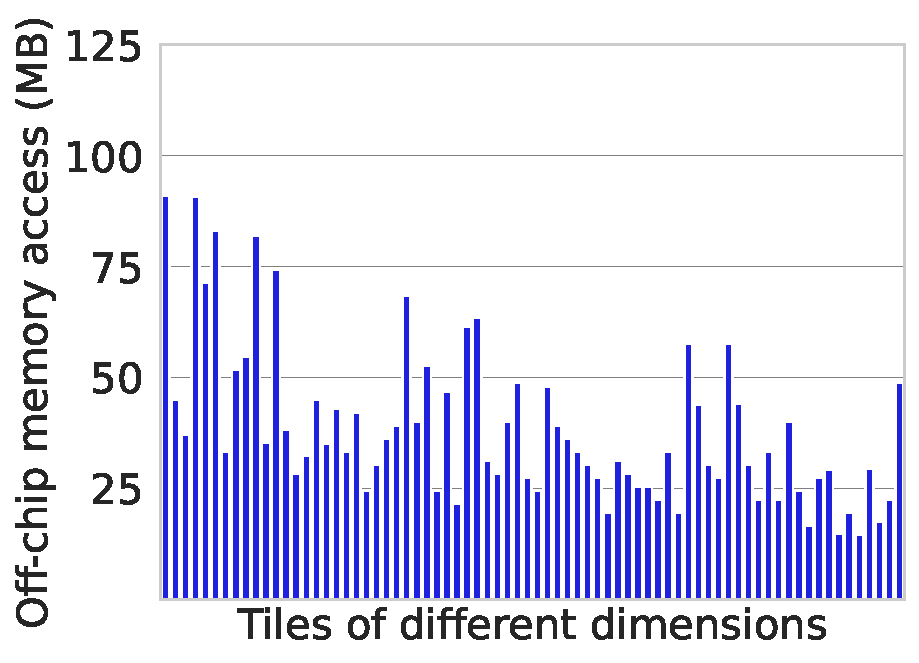
\includegraphics[width=0.4\textwidth]{varyingTileDims.pdf}
		\label{fig:varyingTileDims}}
	\hfil	
	\subfloat[]{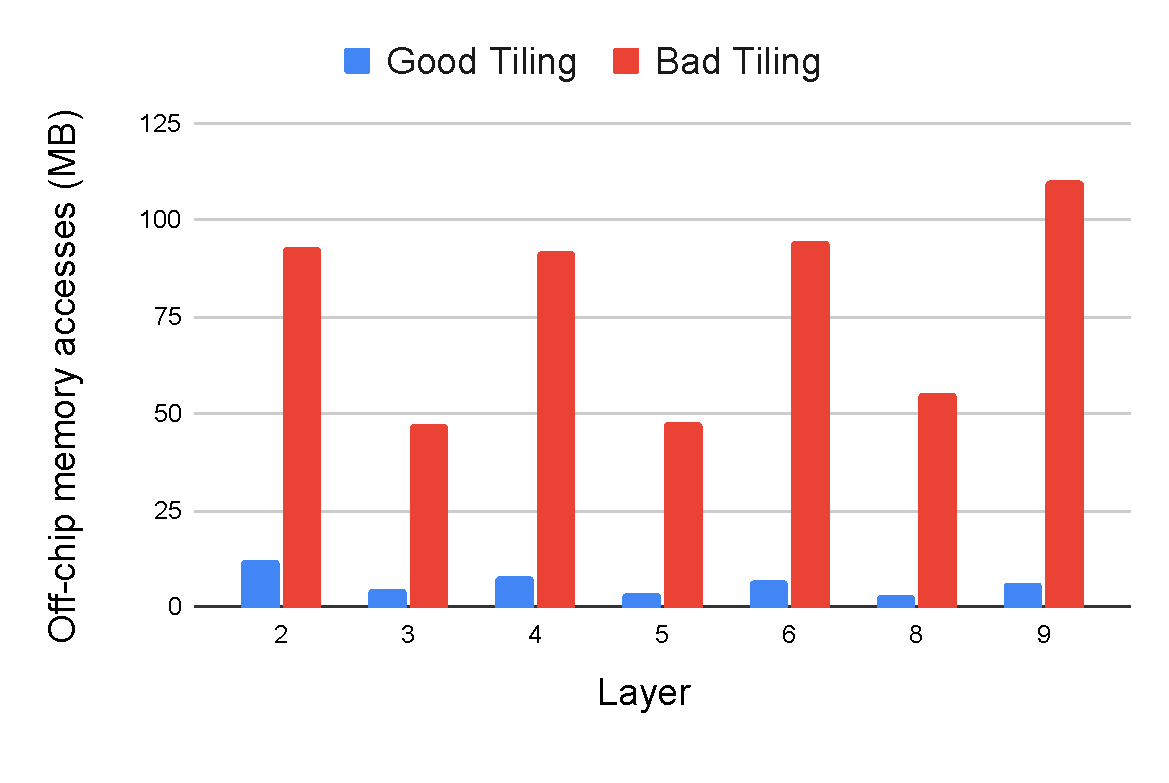
\includegraphics[width=0.4\textwidth]{impactOfTileDims.pdf}
		\label{fig:maxNMinLayerAccess}}
	\hfil	
	\caption{Off-chip memory accesses for 64KB on-chip memory (a) off-chip memory accesses using different tile dimensions for a single layer. (b) Impact of good and bad tile dimensions on different Conv. layers of VGG16.}
	\label{fig:impactOfTileDims}
\end{figure}

Determining the optimal tile dimensions and scheduling scheme requires comparing the off-chip memory accesses for different tile dimensions and scheduling schemes. Modern DNNs have a variety of layers (e.g., convolution, fully connected, recurrent, pooling), each exhibiting different types of data access patterns. Even the layers of the same type differ in shape and size. Due to varying layer shapes, sizes, and types, optimal partitioning, and scheduling vary among layers. Finding the optimal partitioning and scheduling scheme by performing the measurements on the hardware is time-consuming, and large search space makes it practically impossible.

To address this, we have developed an analytical framework that integrates models of NN layers to compute a layer's off-chip memory accesses, data access energy, and the number of compute cycles for mapping a layer on a NN accelerator (Figure~\ref{fig:typicalDNNAccelerator}). Figure~\ref{fig:analyticalModel} shows the block diagram of the analytical framework. The framework is used as a design space exploration engine to find the optimal partitioning and scheduling scheme for a given layer type and layer-shape to optimize NN accelerators' energy efficiency and throughput. 
\begin{figure}[!htb]
	\centering
    \captionsetup{font=sf}	
	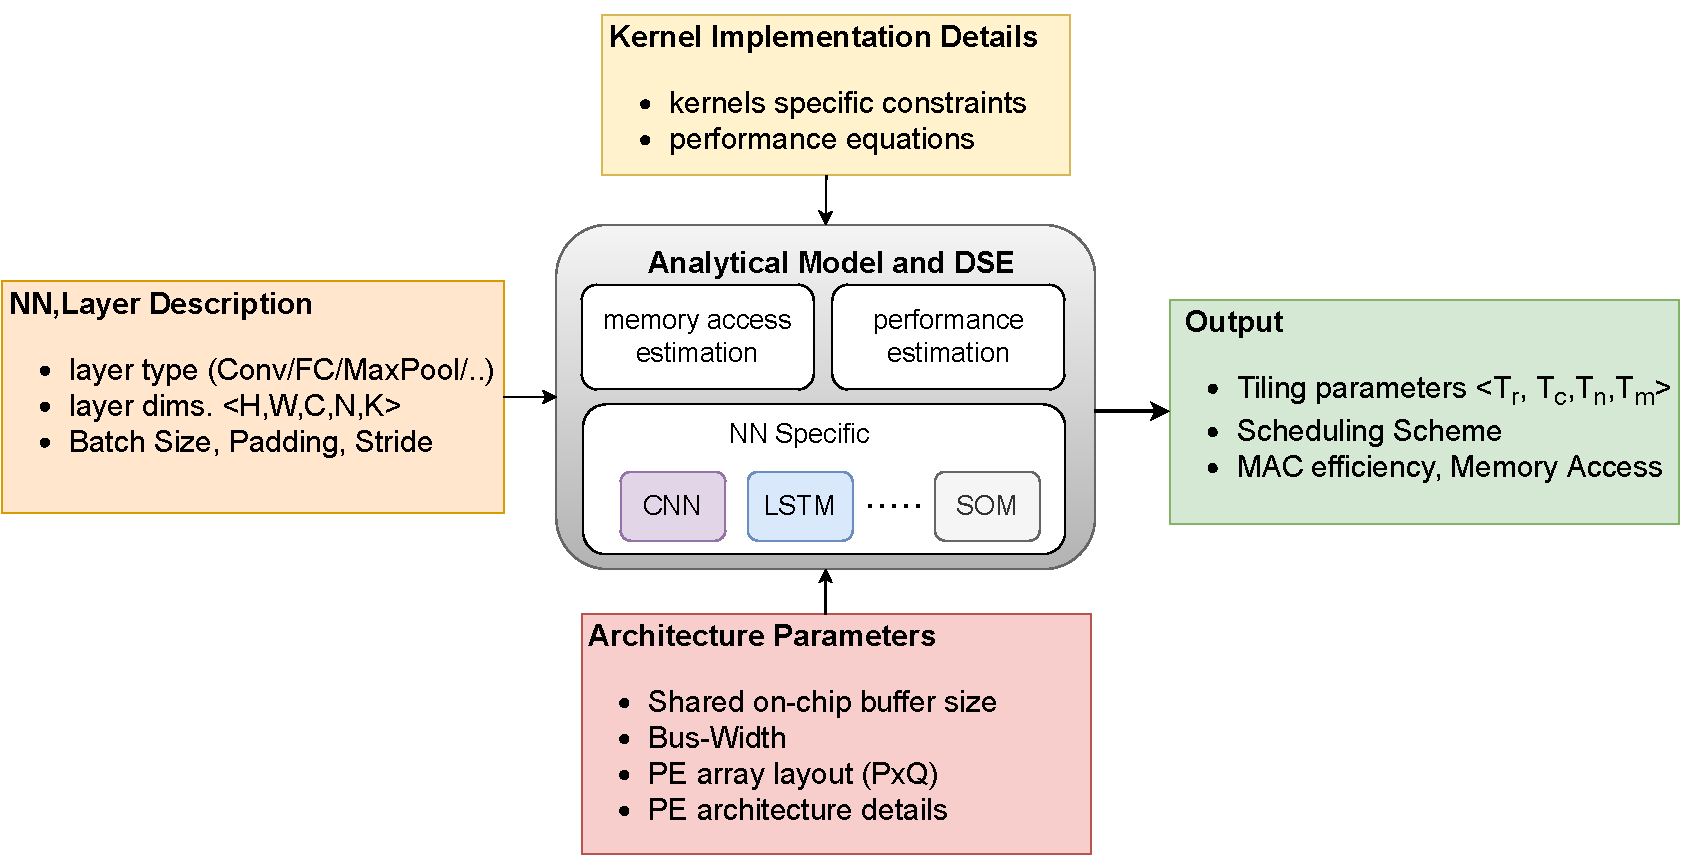
\includegraphics[width=0.9\textwidth]{analyticalModel}
	\caption{Analytical framework to estimate the performance, off-chip memory accesses and energy of DNNs.}
	\label{fig:analyticalModel}
\end{figure}

If a 3D data is partitioned into $N_{tiles}$ number of tiles, $r_t$ is the trips count and $\numBytesOffChip_{t}$ is the number of bytes accessed from off-chip memory for the $t^{th}$ tile, the off-chip memory access of partitioned 3D data can be computed as follows
\begin{align}\label{eq:BasicOffChip3DDataAccess_t}
	\numBytesOffChip_{3D}&{=}\sum_{t=1}^{N_{tiles}}(\numBytesOffChip_{t}{\times}r_t)
\end{align}
In DNN layers, $r_t$ depends on the layer shape, tile dimensions, and scheduling scheme, and it is the same for all the tiles of the 3D data ($r$). However, $B_t$ in equation~\ref{eq:BasicOffChip3DDataAccess_t} varies among the tiles depending on the architectural parameters and address alignment of the tiles. Equation~\ref{eq:BasicOffChip3DDataAccess_t} can be expressed as 
\begin{align}\label{eq:BasicOffChip3DDataAccess}
	\numBytesOffChip_{3D}&{=}r{\times}\sum_{t=1}^{N_{tiles}}\numBytesOffChip_{t}
\end{align}
The analytical framework computes the off-chip memory accesses of a given 3D data using~\eqref{eq:BasicOffChip3DDataAccess}, while considering the data resolution and architectural constraints. The framework considers the bus width and data alignment to compute the off-chip memory accesses precisely. It takes the address and shape of the data as input and iterates for all the tile dimensions. The analytical framework implements models for different layer types and data reuse schemes to compute the memory accesses and data access energy precisely. 

\section{Analytical study of architectural parameters}\label{sec:OffChipAccessModel}
\begin{figure}[!htb]
	\centering
	\captionsetup{font=sf}
	\begin{subfigure}[t]{0.45\textwidth}
		\centering
		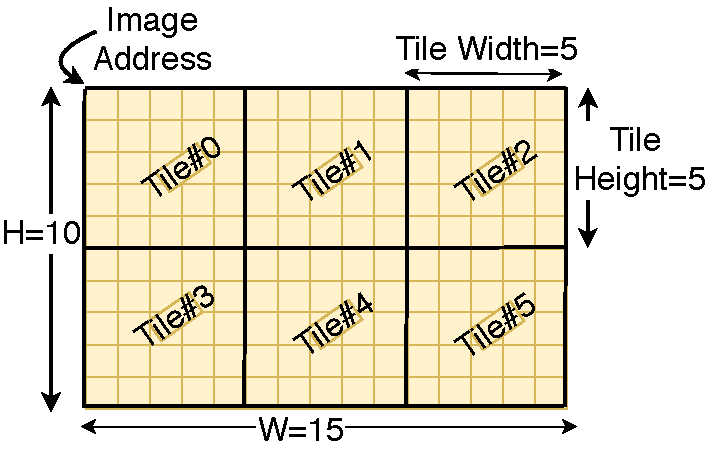
\includegraphics[width=\columnwidth]{A2DImage.pdf}
		\caption{A 2D image and its tiles}
		\label{fig:A2DImage}
	\end{subfigure}
	\hfil
	\begin{subfigure}[t]{0.4\textwidth}
		\centering
		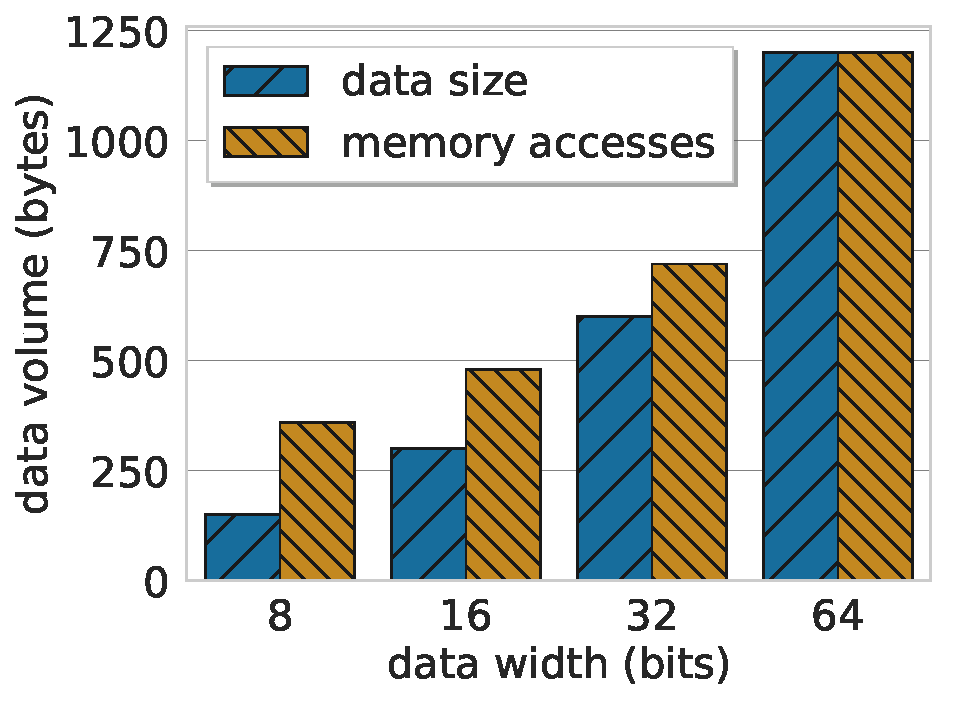
\includegraphics[width=\columnwidth]{MotivationExample.pdf}
		\caption{Data size vs. memory accesses}
		\label{fig:bitPerPixelEffect}
	\end{subfigure}		
	%	\begin{subfigure}[t]{0.3\textwidth}
		%		\centering
		%		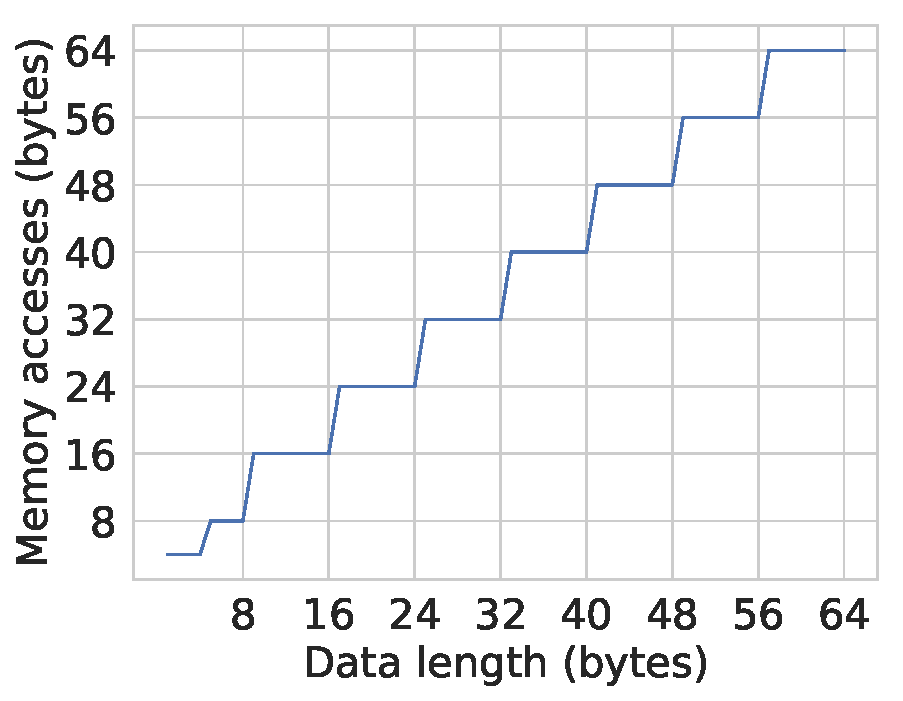
\includegraphics[width=\columnwidth]{Read1To64OnAXI.pdf}
		%		\caption{Memory accesses from aligned address}
		%		\label{fig:OffChipAccessVsLength}
		%	\end{subfigure}
	\caption{A 2D data and memory accesses on 64-bit data bus}
	\label{fig:2DPartitionedData}
	\vspace{-1.0em}	
\end{figure}

3D data of DNN layers and the tiles, into which the layer data is partitioned, is composed of stacked 2D frames. Off-chip memory access of the 3D data and its tiles can be computed by adding the off-chip memory accesses of 2D frames. \figurename{~\ref{fig:A2DImage}} shows an example 2D frame of shape 10$\times$15, partitioned into tiles of dimensions 5$\times$5. Although all tiles have the same size, the off-chip memory accesses for different tiles are not the same. To observe the differences between the tile sizes and off-chip memory accesses of the tiles, we implemented a hardware design using Xilinx SDSoC framework, SDx v2018.3 to access the 2D data stored in DRAM. We measured the memory accesses using AXI Performance Monitor (APM) IP~\cite{APM}, integrated with our design. The target platform is ZedBoard, working at 100MHz frequency, and off-chip memory (DRAM) is accessed using 64 bits AXI bus.  Table~\ref{tab:TileOffChipAccesses} shows the sizes and off-chip memory accesses of each tile on 64 bits wide bus for 8 bits data width. The difference between the tile sizes and the memory accesses is due to the bus width and address alignments of different rows of the tile. 
\begin{table}[h]
	\centering
	\caption{Off-Chip memory accesses of the tiles of size 5$\times$5 }
	\begin{tabular}{|c|c|c|c|c|c|c|c|}
		\hline
		\textbf{Tile\#}& 0  & 1  & 2  & 3  & 4  & 5  & \textbf{Total} \\ \hline
		\textbf{Size(bytes)}& 25 & 25 & 25 & 25 & 25 & 25 & 150   \\ \hline
		\textbf{Mem. Access(bytes)} & 72 & 56 & 56 & 48 & 72 & 56 & 360  \\
		\hline
	\end{tabular}
	\label{tab:TileOffChipAccesses}
\end{table}

\figurename{~\ref{fig:bitPerPixelEffect}} shows the size and off-chip memory accesses of the 2D data shown in  \figurename{~\ref{fig:A2DImage}}, for different data bit widths. For smaller data bit width, the ratio of memory accesses to the data size is higher. Modern NN accelerators use wide memory bus to improve the memory bandwith and low number of bits to represent the data to reduce the storage requirements and memory accesses. Therefore it is crucial to consider the architectural parameters for low resolution data.
\begin{figure}[!htb]
	\centering
	\captionsetup{font=sf}	
	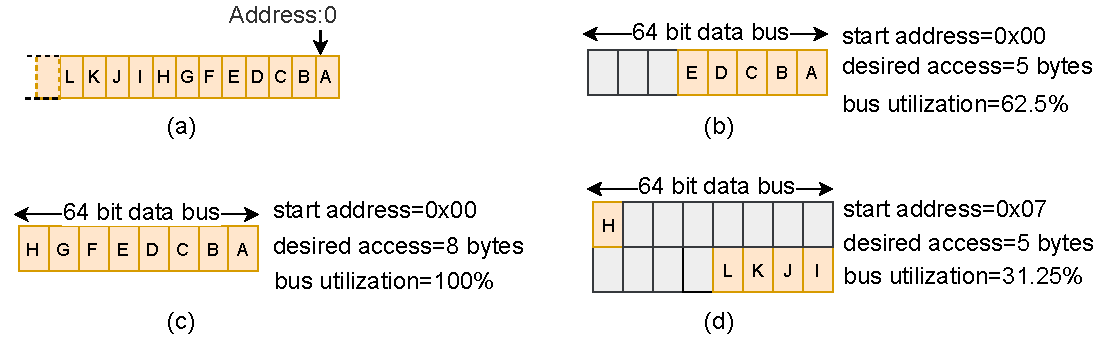
\includegraphics[width=0.9\textwidth]{BurstTranscationOnAXI}
	\caption{Off-chip memory accesses on 64-bit wide data bus}
	\label{fig:AXI_AccesseOn64BitDataBus}
\end{figure}

The DNN accelerators use a wide data bus to access off-chip memory to meet the high memory bandwidth requirement~\cite{Chen2016EyerissAS,chen2014diannao}. If the number of bytes accessed from an off-chip memory address is not a multiple of bus width or the address is not aligned to the word boundary, it results in unused bytes lanes of the data bus. \figurename{~\ref{fig:AXI_AccesseOn64BitDataBus}} illustrates memory accesses on a 64-bit data bus. \figurename{~\ref{fig:AXI_AccesseOn64BitDataBus}a} shows a read transaction of 8 bytes from an aligned address and uses the full bus width. However, if only 5 bytes are read from an aligned address, as shown in \figurename{~\ref{fig:AXI_AccesseOn64BitDataBus}b}, 8 bytes are still accessed. If 5 bytes are read from an unaligned address, it results in 16 bytes of data access, as shown in \figurename{~\ref{fig:AXI_AccesseOn64BitDataBus}c}. The unused byte lanes do not carry any useful data, but they contribute to overall energy consumption. The length of the data read should be chosen such that bus utilization is high and off-chip memory accesses and energy consumption are minimized.

\subsection{Aligned Access}
Number of bytes accessed from off-chip memory ($\numBytesOffChip_{align}$) from aligned addresses for different data length ($\dataLength$) is in multiples of bus width ($\busWidth$), e.g., reading 10 bytes results in 16 bytes of off-chip memory access.  $\numBytesOffChip_{align}$ for $\dataLength$ bytes and bus width $\busWidth$ can be expressed as
\begin{align}\label{eq:alignedAccess}
	\begin{aligned}[b]
		\numBytesOffChip_{align}(\dataLength,\busWidth) = \ceil[\big]{\frac{\dataLength}{\busWidth}}\times {\busWidth}
	\end{aligned}
\end{align}
\subsection{General Case}
To analyze the effect of bus width and address alignment, we express number of bytes accessed from off-chip memory ($\numBytesOffChip$) for $\dataLength$ bytes of data as a function of $\dataLength$, its off-chip memory address ($\addressSym$), and the bus width ($\busWidth$).
The off-chip memory bus protocol supports burst based transactions where multiple data transfers of \emph{transfer size} happen from a starting address~\cite{AxiProtocolSpec}. Most transfers in a transaction are aligned to the \emph{transfer size}. However first transfer may be unaligned to the word boundary. 

The number of bytes accessed from off-chip memory for accessing $\dataLength$ bytes from address $\addressSym$ on $\busWidth$ bytes of bus width can be expressed as
\begin{equation}\label{eq:unalignedAccess}
	\begin{aligned}
		\numBytesOffChip(\addressSym,\dataLength,\busWidth)=(\ceil[\big]{\frac{\addressSym+\dataLength}{\busWidth}}-\floor[\big]{\frac{\addressSym}{\busWidth}})\cdot{\busWidth}
	\end{aligned}
\end{equation}
Equation~\ref{eq:alignedAccess} is a special case of Equation~\ref{eq:unalignedAccess} when memory access is from aligned address.
\section{Off-Chip Memory Access of 3D Data}\label{sec:Access3DData}
\begin{figure}[htb]
	\centering
	\captionsetup{font=sf}
	\begin{subfigure}[t]{0.5\columnwidth}
		\centering
		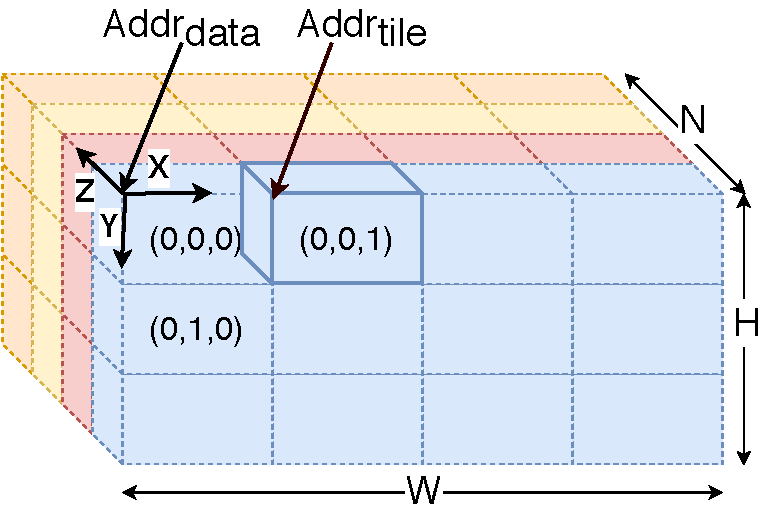
\includegraphics[width=0.6\columnwidth]{3DShapeAndZoomedTile1.pdf}
		\caption{A 3D data partitioned into tiles}
		\label{fig:3dTiledData}
	\end{subfigure}
	\begin{subfigure}[t]{0.4\columnwidth}
		\centering
		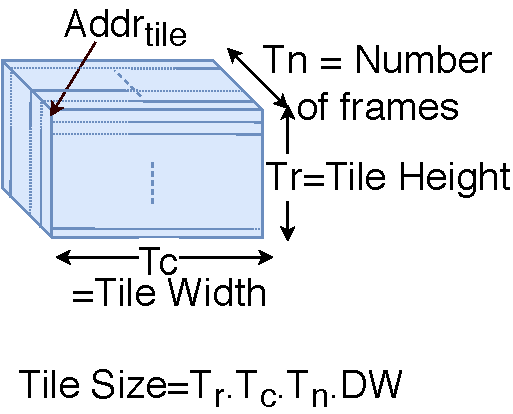
\includegraphics[width=0.6\columnwidth]{SingleTile.pdf}
		\caption{A 3D tile}
		\label{fig:3dTile}
	\end{subfigure}
	\caption{Off-Chip Accesses and a 3D partitioned data and tiles}
	\label{fig:3DPartitionedData}
\end{figure}
Consider a 3D data of shape $\langle W,H,N\rangle$, partitioned into tiles of dimension $\langle T_c,T_r,T_n\rangle$ as shown in  Fig.~\ref{fig:3dTiledData} and Fig.~\ref{fig:3dTile}. Each tile is identified by index $(x,y,z)$ where $x, y, z \in \mathbb{Z}$ and 
\begin{align}\label{eq:TileIndexing}
	\begin{aligned}
		0\leq &x<\ceil[\big]{\frac{W}{T_c-\numOverlap}}, \\
		0\leq &y<\ceil[\big]{\frac{H}{T_r-\numOverlap}}, \\
		0\leq &z<\ceil[\big]{\frac{N}{T_n}}
	\end{aligned}
\end{align}
$\numOverlap$ is the number of elements or rows overlapping between adjacent tiles.

Algorithm~\ref{Algorithm1} computes the number of bytes accessed from off-chip memory for the 3D data. Each data element is represented by $DW$ bytes. The algorithm takes the address of the data ($Addr_{data}$), tile dimensions, data shape, and $\numOverlap$ as input and iterates lines~\ref{alg:ForAllTilesLoopk}--\ref{alg:loopkEnd} for all the tiles. It computes indices of the first element of the tile in the 3D array of the data using the tile index $(x,y,z)$ and $\numOverlap$ in lines~\ref{alg:idxc}--\ref{alg:idxn}. Using the indices of the first element it computes the address of the tile in line~\ref{alg:tileAddr}, and dimensions of the tile in line~\ref{alg:tileDim}. The algorithm computes the total number of bytes accessed from off-chip memory by accumulating the number of bytes accessed for each tile in line~\ref{alg:tileAcc}. 

The address of the tile in line~\ref{alg:tileAddr} is computed by the function GetTileAddr using equation~\ref{eq:TileAddress} below
\begin{align}\label{eq:TileAddress}
	\begin{split}
		%&Addr_{tile}=Addr_{data} + z\cdot T_{n}\cdot H \cdot W + y\cdot T_{r}\cdot W + x\cdot T_{c} \\
		GetTileAddr(Addr_{data},c,r,n,\langle W,H,N\rangle){=}Addr_{data} + c + r\cdot W + n\cdot W\cdot H
	\end{split}
\end{align}
If the data dimensions are not multiples of corresponding tile dimensions, the tiles at the border of the data (e.g., the right-most or bottom-most tiles) will have smaller dimensions. The function GetTileDim computes the dimensions of the tiles.

The function GetTileAcc in Lines~\ref{alg:FuncTileAccess}--\ref{alg:FuncTileAccessEnd} computes the addresses and number of bytes ($contSz$) for each off-chip memory transaction. $contSz$ is the number of contiguous bytes to access in a transaction. Let $T_n$ is the number of frames in the tile. If the tile width ($T_c$) is the same as the data width ($W$) (line~\ref{alg:TileAccessIf2}), then all the data elements of $T_r$ rows of a frame are contiguous, and the complete tile can be accessed using $T_n$ number of addresses. If the condition in line~\ref{alg:TileAccessIf1} is true, then all elements of the tile are contiguous and can be accessed using a single transaction of $T_c\cdot T_r\cdot T_n\cdot DW$ bytes (line~\ref{alg:TileAccessSingleTxn}). In all other cases, the tile is accessed using row addresses computed in line~\ref{alg:TileRowAddr}. The function computes the number of bytes accessed from off-chip memory for a tile ($Acc_{tile}$) in lines~\ref{alg:TileAccessIf1End},~\ref{alg:TileAccess2}, and~\ref{alg:TileAccessFor2End} using ~\eqref{eq:unalignedAccess}. 
\begin{algorithm}[H]
	\caption{BW Aware off-chip memory access}
	 \label{Algorithm1}
	 \begin{algorithmic}[1]
	 	\Procedure{BWA}{$Addr_{data},\langle T_c,T_r,T_n\rangle,\langle W,H,N\rangle,\numOverlap$} \label{alg:BWA}
	 	\State $Acc_{data}\gets 0$
	 	\State $Addr_{tile}\gets Addr_{data}$
        \For{$x,y,z\leftarrow (0,0,0)$ ~\textbf{to} $(\ceil[\big]{\frac{W}{T_c-\numOverlap}}{-}1,\ceil[\big]{\frac{H}{T_r-\numOverlap}}{-}1,\ceil[\big]{\frac{N}{T_n}}{-}1)${\label{alg:ForAllTilesLoopk}}}
        \State $c\gets x\cdot (T_c-\numOverlap)$\label{alg:idxc}
        \State $r\gets y\cdot (T_r-\numOverlap)$\label{alg:idxr}
        \State $n\gets z\cdot T_n$\label{alg:idxn}
        \State $Addr_{tile}\gets \Call{GetTileAddr}{Addr_{data},c,r,n,\langle W,H,N\rangle}$\label{alg:tileAddr}
        \State $\langle T_c^1,T_r^1,T_n^1\rangle\gets$ \Call{GetTileDim}{$c,r,n,\langle T_c,T_r,T_n\rangle,\langle W,H,N\rangle$}\label{alg:tileDim}
        \State $Acc_{data}\gets Acc_{data}+$ \Call{GetTileAcc}{$Addr_{tile},\langle T_c^1,T_r^1,T_n^1\rangle,\langle W,H,N\rangle$}\label{alg:tileAcc}
	 	\label{alg:UpDiag_ReuseR2}   
	 	\EndFor \label{alg:loopkEnd}
	 	\State \textbf{return} $Acc_{data}$
	 	\EndProcedure
	 	
	 	\Procedure{GetTileAcc}{Addr$_{tile}$,$\langle T_c,T_r,T_n\rangle$,$\langle W,H,N\rangle$} \label{alg:FuncTileAccess}
	    \State $Acc_{tile}\gets 0$
	    \If{$T_c = W$ {\bf and} $T_r=H${\label{alg:TileAccessIf1}}}
	    	\State$contSz\gets T_c\cdot T_r\cdot T_n\cdot DW$\label{alg:TileAccessSingleTxn}
	    	\State$Acc_{tile}{\gets}$$\numBytesOffChip({Addr_{tile},contSz,BW})$\label{alg:TileAccessIf1End}
	    \Else
	    	    \For{$f\leftarrow 1$ ~\textbf{to} $T_n${\label{alg:TileAccessFor1}}}
	    	       \State Addr$_{f}{\gets} Addr_{tile}{+}(f{-}1){\cdot}H{\cdot}W$\label{alg:TileAccessFrameAddr}
	    	       \If{$T_c = W${\label{alg:TileAccessIf2}}}
   					    \State $contSz{\gets}T_c\cdot T_r\cdot DW$
                        \State $Acc_{tile}{\gets}Acc_{tile}+$$\numBytesOffChip({Addr_f,contSz,BW})$\label{alg:TileAccess2}
	    	       \Else
	    	           \State $contSz{\gets}T_c{\cdot}DW$
	    	           \For{$r\leftarrow 1$ ~\textbf{to} $T_r${\label{alg:TileAccessFor2}}}
                            \State $Addr_{(f,r)}{\gets}Addr_{f}+(r-1)\cdot W$\label{alg:TileRowAddr}
                            \State $Acc_{tile}{\gets}Acc_{tile}+$$\numBytesOffChip({Addr_{(f,r)},contSz,BW})$\label{alg:TileAccessFor2End}
	    	           \EndFor
	    	       \EndIf
	            \EndFor	
	    
	    \EndIf
	    \label{alg:FuncTileAccessEnd}	 	
	 	\State \textbf{return} $Acc_{tile}$
	 	\EndProcedure	
	
	
	 	\Procedure{GetTileDim}{$c,r,n$,$\langle T_c, T_r,T_n\rangle$,$\langle W,H,N\rangle$} \label{alg:FuncTileDimEnd}
	 	\State $T^1_c\gets min(T_c,W-c)$
	 	\State $T^1_r\gets min(T_r,H-r)$
	 	\State $T^1_n\gets min(T_n,N-n)$
	 	\State \textbf{return} ${\langle T^1_c,T^1_r,T^1_n\rangle}$
	 	\EndProcedure

	\end{algorithmic}
\end{algorithm}
DNN accelerators access layer data (ifm, ofm, and weights) partitioned into tiles. The tile dimensions should be chosen carefully to minimize the transfer of extra bytes to reduce off-chip memory access. We have proposed a bus width aware approach (BWA) that factors in the architectural parameters to precisely compute the off-chip memory access of 3D tiles and the layer data.

Figure~\ref{fig:measVsEst} shows the comparison between the off-chip memory accesses estimated by the analytical framework and measurements performed on Xilinx FPGA for different layers of varying shapes and sizes of a popular CNN, VGG16. The experimental results on popular CNNs, AlexNet, and VGG16, show that the difference between estimated and measured off-chip memory accesses is less than 4\%. The framework is also helpful in analyzing the layer-wise distribution and breakdown of memory accesses, as shown in Figure~\ref{fig:ifmOfmWtsDistribution}. The proposed framework is a valuable tool for quickly analyzing the memory accesses and data access energy for different tile dimensions, and data reuse schemes to search for the optimal solution. 
\begin{figure}[!htb]
	\centering
	\captionsetup{font=sf}
	\subfloat[]{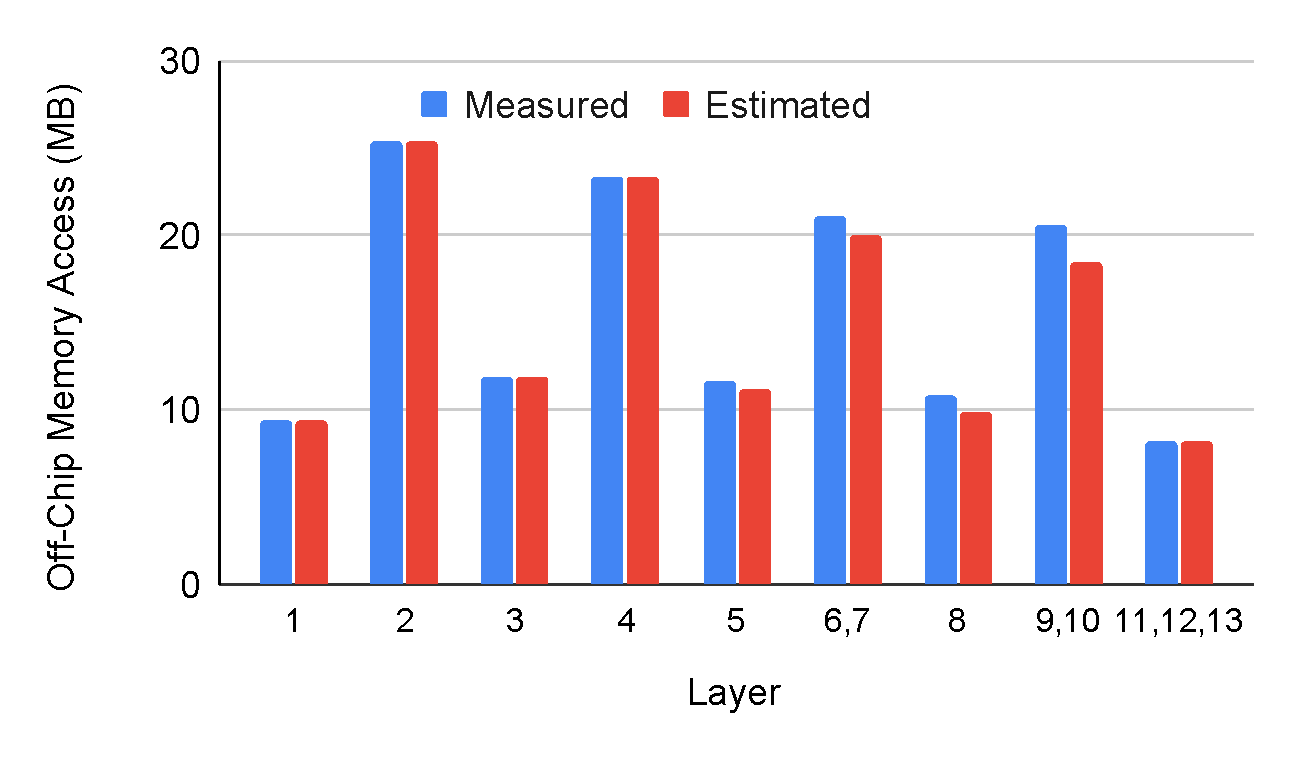
\includegraphics[width=0.4\textwidth]{measuredVsEstimated.pdf}
		\label{fig:measVsEst}}
	\hfil
	\subfloat[]{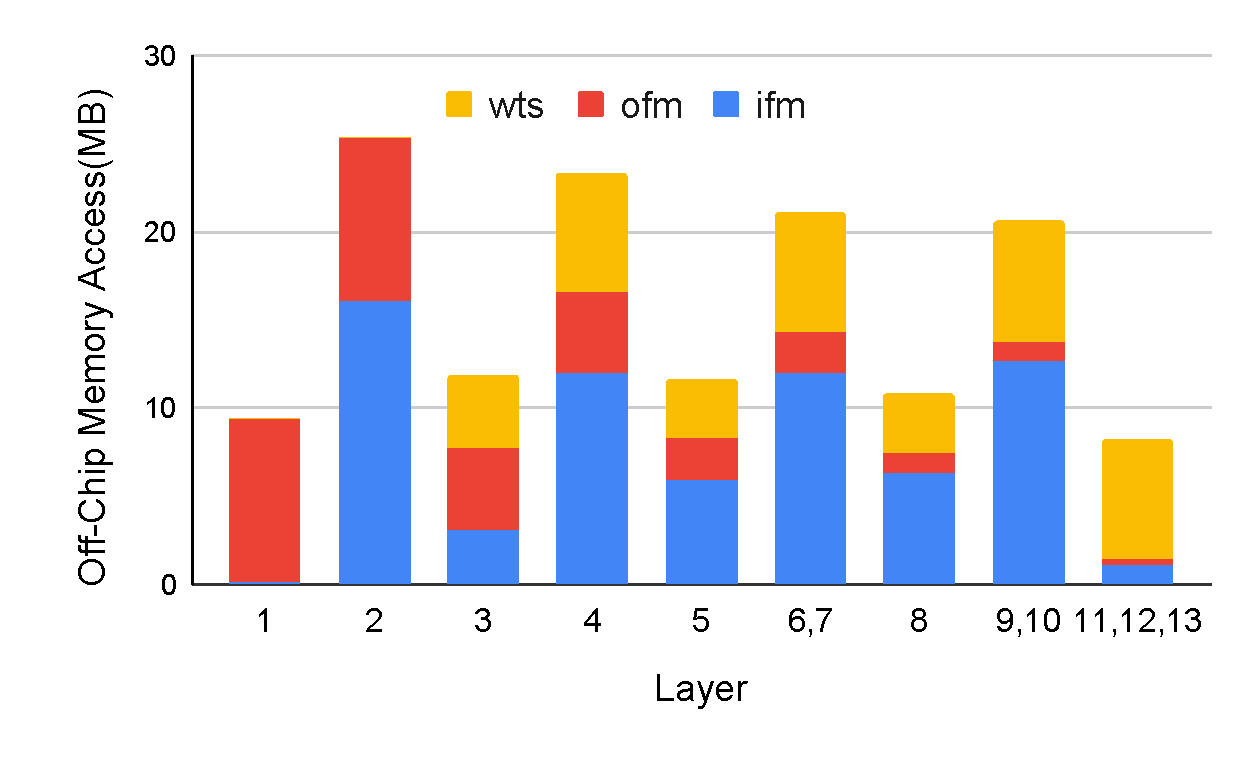
\includegraphics[width=0.4\textwidth]{memAccessDistribution.pdf}
		\label{fig:ifmOfmWtsDistribution}}
	\hfil   
	\caption{Off-chip memory accesss of VGG16 layers (a) Comparison between the analytical framework and hardware measurements. (b) Breakdown by data type using analytical framework.}
	\label{fig:nnLayerData}
\end{figure}
